\setcounter{section}{21}
\section{Двоичная куча}

\textbf{Опр} Куча (двоичная куча) - это древовидная структура данных, для которой выполняются следующие условия:
 ~~\begin{itemize}
        \item Значение в любой вершине не меньше, чем значения ее потомков (maxHeap), значение в любой вершине не больше, чем значения ее потомков (minHeap)
        \item Глубина листьев (расстояние до корня) отличается не более чем на один
        \item Последний слой заполняется слева направо
    \end{itemize}
    
\textbf{Опр} Глубина кучи - максимальное расстояние от корня до листа. Глубина кучи (высота дерева) = O(log(n)), где n - количество элементов.

\begin{figure}[h]
\center{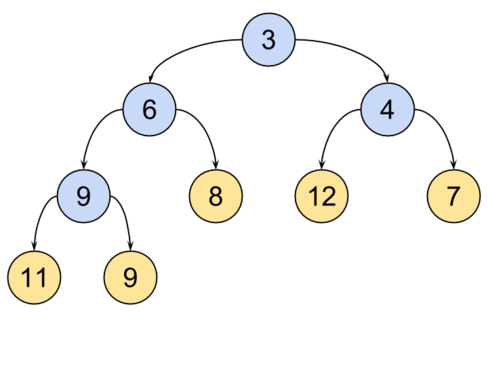
\includegraphics[width=5cm]{images/22_1}}
\caption {minHeap}
\label{ris:image}
\end{figure}
    
\textbf{ Куча должна уметь поддерживать следующие операции}:
    ~~\begin{itemize}
        \item insert( x ) - вставка элемента в кучу
        \item getMax() - вывести максимальный элемент (для maxHeap), getMin() - вывести минимальный элемент (для minHeap)
        \item extractMax() - удалить максимальный элемент (для maxHeap), extractMin() - удадить минимальный элемент (для minHeap)
        \item decreaseKey( ptr, $\delta$ ) - уменьшение элемента по указателю ptr на $\delta$ (опционально)
    \end{itemize}
    
\textbf{Замечание:} Все операции в куче должны делаться за О( log n ).

\textbf{Реализация кучи на массиве}

Удобнее всего двоичную кучу хранить в виде массива a[0..n-1], у которого нулевой элемент, a[0] — элемент в корне, а потомками элемента a[i] являются a[2i+1] и a[2i+2].
 \begin{figure}[h]
\center{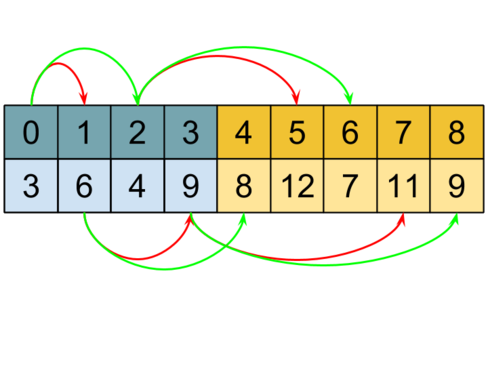
\includegraphics[width=5cm]{images/22_2} }
\caption {Красная стрелка - левый сын, зеленая - правый сын}
\label{ris:image}
\end{figure}

\section{Операции siftDown и siftUp. Корректность}
\textbf{Замечание:} будем рассматривать minHeap

Для того чтобы поддерживать кучу корректной введем две функции siftDown и siftUp.

\textbf{siftDown} - буквально, просеивание вниз. Эта операция перемещает элемент на более \textbf{низкие} уровни, пока не восстановится свойство кучи (оба ребенка не меньше самого элемента).

\textbf{siftDown}:

 \begin{lstlisting}
    void Heap::siftDown(int i) {
    int leftChildIndex = 2 * i + 1;
    int rightChildIndex = 2 * i + 2;
    int bigChildIndex = i;

    while (2*i + 1 < size) {
        leftChildIndex = 2 * i + 1;
        rightChildIndex = 2 * i + 2;
        minIndex = i;
        
        if (a[leftChildIndex] < a[minIndex])
            minIndex = leftChildIndex;
        if (rightChildIndex < size &&
        a[rightChildIndex] < a[minIndex])
            minIndex = rightChildIndex;

        if (minIndex == i) break;

        swap(a[i], a[minIndex]);
        i = minIndex;

    }


}
\end{lstlisting}

\textbf{
Лемма (доказательство корректности siftDown):}

Пусть в дереве выполняются все неравенства между детьми и родителями, кроме, может быть, одного элемента $a_{i}$, для которого $a_{i}$ > $a_{2i + 1}$ и (или) $a_{i}$ > $a_{2i+2}$. Тогда после выполнения операции siftDown корректность восстановится.

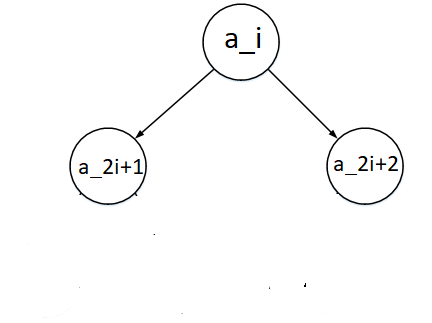
\includegraphics[width=5cm]{images/23_1}

$\blacktriangle $ Рассмотрим 5 случаев взаимного соотношения элементов $a_{i}$ ,$a_{2i+1}$, $a_{2i+2}$.
\begin{itemize}
    \item[1] $a_{i}$ <= $a_{2i + 1}$ и $a_{i}$ <= $a_{2i+2}$. Тогда мы заходим в цикл, но ни в первое, ни во второе условие не попадаем, minIndex остается равным i, и мы выходим из функции. Дерево корректно.
    
    \item[2] $a_{i}$ > $a_{2i + 1}$ и $a_{i}$ <= $a_{2i+2}$. Тогда мы заходим в цикл, а после в первое условие. minIndex = leftChildIndex. Во второе условие мы не заходим, в третье тоже. Меняем местами левого ребенка и родителя. Тогда новый родитель больше обоих детей. Тут все корректно. Т.к. оба поддерева изначально были корректны, то мы могли что-то нарушить только в левом поддереве. Идем туда.
     \item[3]$a_{i}$ <= $a_{2i + 1}$ и $a_{i}$ > $a_{2i+2}$. Рассуждения аналогичны расссуждению в п.2.
     \item[4] $a_{i}$ > $a_{2i + 1}$ и $a_{i}$ > $a_{2i+2}$. Тут мы заходим в цикл, а после сразу попадаем в первое условие. minIndex = leftChildIndex.
     Если правый ребенок меньше левого, то он будет новым родителем, т.к. в этом случае правый ребенок является минимальным элементном из трех. Иначе - левый ребенок минимальный. И он станет новым родителем. Меняем родителя с минимальным из детей и идем дальше, нужно проверить, не нарушили  ли мы что-то в ветке, в которой был минимальный ребенок.
     
    \item[5] Если детей нет, в цикл не заходим, все корректно, функция завершает работу. Если есть только один ребенок, то сравнение происходит только с ним. $\blacksquare$
     \end{itemize} 
     
    \textbf{siftUp} - буквально, просеивание вверх. Эта операция перемещает элемент на более \textbf{высокие} уровни, пока не восстановится свойство кучи (оба ребенка не меньше самого элемента). 

\textbf{siftUp}:
\begin{lstlisting}
void Heap::siftUp(int i) {
    int parentIndex = (i - 1) / 2;
    while (i > 0 && a[i] > a[parentIndex]) {
        swap(a[i], a[parentIndex]);
        i = parentIndex;
        parentIndex = (i - 1) / 2;

    }
}
\end{lstlisting}
\textbf{
Лемма (доказательство корректности siftUp):}

Пусть в дереве выполняются все неравенства между детьми и родителями, кроме, может быть, одного элемента $a_{i}$, для которого  $a_{i}$ > $a_{(i-1)/2}$ Тогда после выполнения операции siftUp корректность восстановится.

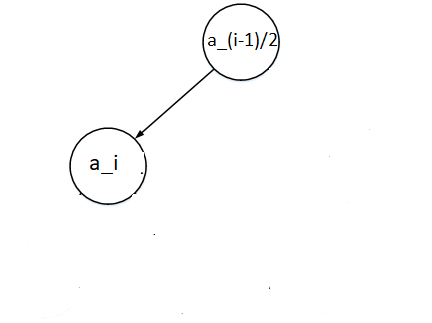
\includegraphics[width=5cm]{images/23_2}

$\blacktriangle$ Рассмотрим 2 случая:
\begin{itemize}
\item[1] Если элемент корневой или $a_{i}$ <= $a_{(i-1)/2}$ тогда дерево корректно, и в цикл мы не заходим, функция завершает выполнение.
\item[2] Если $a_{i}$ > $a_{(i-1)/2}$, то меняем местами родителя и ребенка. Новый родитель не увеличивается, поэтому неравенства между новым родителем и другим ребенком остаются корректными, при этом восстанавливаются неравенства между родителем и двумя детьми. В поддеревьях все ок. Но могло что-то нарушиться выше, поэтому текущий родитель становится ребенком, и процесс повторяется. $\blacksquare$
\end{itemize} 

\section{Выражение insert(x), getMin(), extractMin() и decreaseKey(ptr, $\delta$) через siftUp() и siftDown(). Асимптотика этих операций}
\subsection*{Асимптотика операций siftUp() и siftDown()}

Выполняя операции siftUp() и siftDown() мы переходим между уровнями, на каждом из которых выполняем C = const количество операций. Высота дерева - log(n), поэтому каждая из операций выполняется за время, не превосходящее C*log(n). Таким образом асимптотика O(log(n)).

\subsection*{Основные операции:}

\textbf{Insert: }
 \begin{lstlisting}
void Heap::insert(int x) {
    a.push_back(x); 
    size++; 
    siftUp(size - 1); 
}
\end{lstlisting}
Вставляем элемент в конец. Тогда могли нарушиться только неравенства с родителем. Поэтому необходимо просеять наверх. \textit{Асимптотика: O(log(n)) за счет выполнения операции siftUp()}

\textbf{GetMin: }
 \begin{lstlisting}
int Heap::getMin() { 
    return a[0]; 
}
\end{lstlisting}
Минимальный элемент кучи лежит в вершине дерева, просто его выводим. \textit{Асимптотика: O(1)}

\textbf{ExtractMin: }
 \begin{lstlisting}
void Heap::extractMin() {
    a[0] = a[size - 1]; 
    a.pop_back();
    size--;
    siftDown(0);
}
\end{lstlisting}
Меняем первый элемент и последний местами, удаляем последний. Т.к. у первого элемента нет родителей, то неравенства могли нарушиться только с детьми, поэтому просеиваем элемент вниз.\textit{ Асимптотика: O(log(n)) за счет выполнения операции siftDown()}

\textbf{DecreaseKey:
}

Переходим по указателю на элемент и уменьшаем его на $\delta$. Понятно, что в поддеревьях неравенства не нарушились, поэтому необходимо восстановить только неравенства с родителями. Поэтому делаем siftUp от этого элемента.\textit{ Асимптотика: O(log(n)) за счет выполнения операции siftUp()}

\section{Построение кучи (heapify) за линейное время (сходимостью ряда можно пользоваться б/д).}
\textbf{Алгоритм построения: }

Заполняем массив, как он поступил во входных данных. Заметим, что элементы на последнем уровне не нуждаются в упорядочивании, поэтому нам необходимо упорядочить только первые n/2 элементов. Будем каждый элемент, начиная с n/2, просеивать вниз. И в результате получим кучу.

\textbf{Корректность построения:}

$\blacktriangle$ До вызова siftDown для вершины, ее поддеревья являются кучами. После выполнения siftDown эта вершина с ее поддеревьями будут также являться кучей. Значит, после выполнения всех siftDown получится куча. $\blacksquare$

\begin{lstlisting}
void Heap::heapify() {
    for (int i = size / 2 - 1; i >= 0; --i) {
        siftDown(i);
    }
}
\end{lstlisting}
\textbf{Асиптотика: O(n). Доказательство}

$\blacktriangle$

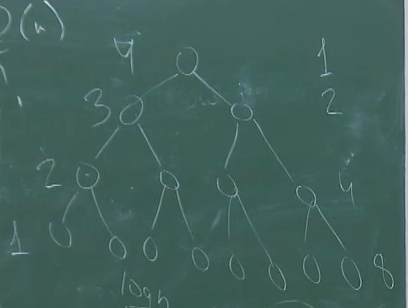
\includegraphics[width=5cm]{images/25}
 
  $\displaystyle\sum_{h=1}^{\log_{2}{n}} h*2^{\log_{2}{n} - h}$ = $n*\displaystyle\sum_{h=1}^{\log_{2}{n}} \frac{h}{2^h}$
 
 $\displaystyle\sum_{h=1}^{\log_{2}{n}} \frac{h}{2^h}$ сходится к 2. 
 Таким образом T(n) = 2*n. Асимптотика O(n).
 $\blacksquare$


\section{Биномиальное дерево, биномиальная куча: определение.}

\textbf{Опр} Биномиальное дерево $T_{k}$ (англ. binomial tree) - дерево, определяемое для каждого k= 0,1,2,... следующим образом: $T_{0}$ - дерево, состоящее из одного узла; $T_{k}$ состоит из двух биномиальных деревьев $T_{k-1}$, связанных вместе таким образом, что корень одного из них является дочерним узлом корня второго дерева.

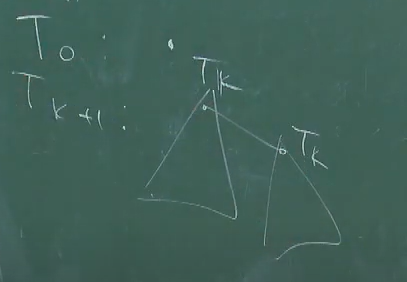
\includegraphics[width=5cm]{images/26_1}
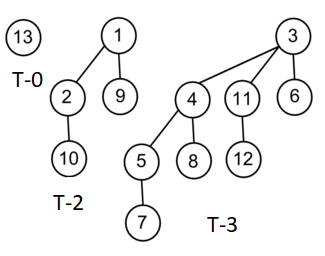
\includegraphics[width=5cm]{images/26_2}

\textbf{Опр} Биномиальная куча - это несколько биномиальных деревьев попарно различных порядков. Например, ($T_{1}$, $T_2$, $T_4$ - куча. $T_{1}$, $T_2$, $T_2$ - не куча)

При этом каждое биномиальное дерево в куче подчиняется свойству неубывающей кучи: ключ узла не меньше ключа его родительского узла

\textbf{Утверждение:} Биномиальное дерево $T_k$ имеет $2^k$ вершин.

$\blacktriangle$
Докажем по индукции:
\begin{itemize}
    \item[1] База k=1 — верно.
    \item[2] Пусть для некоторого k условие верно
    \item[3] Для k+1: Так как в дереве порядка k+1 вдвое больше узлов, чем в дереве порядка k, то дерево порядка k+1 имеет $2^{k}*2=2^{k+1}$ узлов. Переход доказан, следовательно биномиальное дерево $T_k$ имеет $2^{k}$ вершин.
    $\blacksquare$
\end{itemize}

\textbf{Следствие:} Максимальный порядок дерева биномиальной кучи не превосходит log(n)

\textbf{Утверждение:} Биномиальное дерево $T_k$ с n вершинами имеет высоту k.

$\blacktriangle$
Докажем по индукции:
\begin{itemize}
    \item[1] База k=1 — верно
    \item[2]  Пусть для некоторого k условие верно
     \item[3] Для k+1: Так как в дереве порядка k+1 высота больше на 1 (так как мы подвешиваем к текущему дереву дерево того же порядка), чем в дереве порядка k, то дерево порядка k+1 имеет высоту k+1.    $\blacksquare$
\end{itemize}

\section{Операции merge, insert, getMin, extractMin и decreaseKey в биномиальной куче.
Доказательство корректности и времени работы.}

\textbf{Getmin: }

Для нахождения минимального элемента надо найти элемент в списке корней с минимальным значением.

\textit{Асимптотика: Так как корней в этом списке не более [log(n)]+1, то операция выполняется за O(log(n)).}
При вызове этой процедуры для кучи, изображенной на картинке ниже, будет возвращен указатель на вершину с ключом 1.

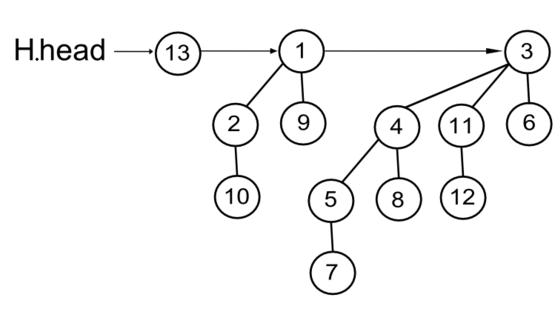
\includegraphics[width = 5cm]{images/27_1}

\textbf{DecreaseKey: }

Так же, как и в обычкой куче, необходимо уменьшить элемент по указателю, а потом просеить вверх с помощью операции siftUp().

\textit{Асимптотика: как и в обычной куче, decreaseKey работает за глубину дерева. Порядок деревьев в биномиальной куче из n элементов не превосходит log(n), высота биномиального дерева равна его порядку, поэтому асимптотика работы decreaseKey O(log(n)) }

\textbf{Merge: }
Эта операция избавляет биномиальную кучу от повторяющихся порядков древьев. 

Пусть есть две биномиальные кучи с H и H1, которые мы хотим склеить в одну. Пусть максимальный порядок среди этих деревьев m. 
\begin{itemize}
    \item[1] Идем циклом от 0 до m.
    \item[2] Если $T_i$ есть в обоих кучах, то сливаем их в $T_i+1$, просто выбирая из вершин этих деревьев минимальную и подвешивая к ней второе дерево.
\end{itemize}

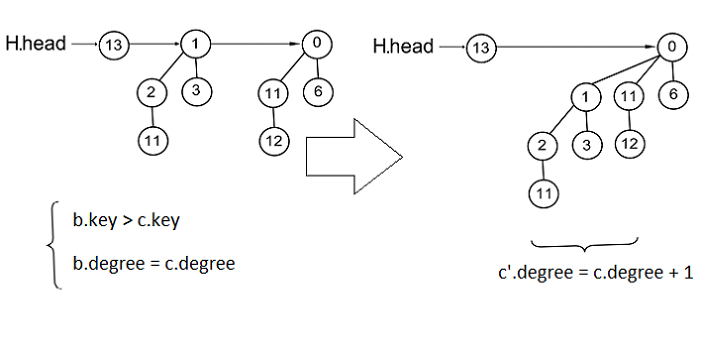
\includegraphics[width = 5cm]{images/27_2}

\textit{Асимптотика: Слияние двух биномиальных деревьев равного порядка происходит за О(1), число таких слияний не превосходит максимального порядка дерева в куче, т.е. log(n). Таким образом, асимптотика O(log(n)).}

\textbf{Корректность:} 

$\blacktriangle$
\begin{itemize}
    \item Корректность слияния двух биномиальных деревьев равного подядка k: оба дерева корректны, после операции по определению получается корректное дерево k+1 порядка, причем за счет того, что к меньшей вершине подвешивается большая, сохраняется основное свойство кучи.
    \item Корректность самого merge: На каждом этапе мы проверяем, нет ли деревьев одинакового порядка, начиная с дерева 0 порядка, и избавляемся от совпадений. Поскольку слиянием двух деревьев мы не можем получить деревья меньшего порядка, то среди деревьев меньшего порядка не может внезапно появиться двух деревьев совпадающего порядка, поэтому, когда мы дойдем до конца цикла, получим корректную кучу. $\blacksquare$
    
\end{itemize}

\textbf{Insert:}

Чтобы добавить новый элемент в биномиальную кучу нужно создать биномиальную кучу H1 с единственным узлом, содержащим этот элемент, за время O(1) и объединить ее с биномиальной кучей H за O(log(n)), так как в данном случае куча H1 содержит лишь одно дерево. \textit{Асимптотика O(log(n))}

 \textbf{Корректность:} Поскольку операция merge корректна, а H1 - корректная биномиальная куча, то вся операция вставки корректна.

\textbf{ExtractMin:
}

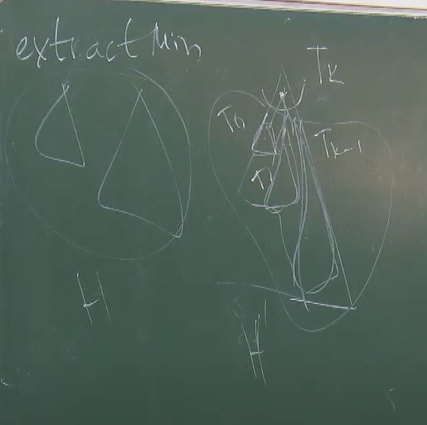
\includegraphics[width = 5cm]{images/27_3}

Пусть изначально имеем биномиальную кучу H
\begin{itemize}
\item Найдем биномиальное дерево с минимальным корневым значением. Предположим, что это дерево $T_k$. Время работы этого шага алгоритма O(log(n)).
\item Удаляем дерево $T_k$ из кучи H. Иными словами, удаляем его корень из списка корней кучи. Это можно сделать за время O(1).

\item Пусть H1 — куча детей найденного корня. Эта куча корректна, поскольку все сыновья родительского удаленного узла имели различный порядок. После этого сливаем кучу H1 c H за О(log(n)).
\end{itemize}
\textit{Таким образом, асимптотика работы алгоритма: O(log(n))}

\section{Сортировка кучей (Heap Sort). Несуществование кучи (основанной на сравнениях), обрабатывающей insert и extractMin за O(1).}

\subsection*{Сортировка кучей. Алгоритм}

Необходимо отсортировать массив A, размером n. Построим на базе этого массива за O(n) кучу для максимума. Так как максимальный элемент находится в корне, то если поменять его местами с A[n-1], он встанет на своё место. Далее вызовем процедуру siftDown(0), предварительно уменьшив heapSize на 1. Она за O(log(n)) просеет A[0] на нужное место и сформирует новую кучу (так как мы уменьшили её размер, то куча располагается с A[0] по A[n-2], а элемент A[n-1] находится на своём месте). Повторим эту процедуру для новой кучи, только корень будет менять местами не с A[n-1], а с A[n-2]. Делая аналогичные действия, пока heapSize не станет равен 1, мы будем ставить наибольшее из оставшихся чисел в конец не отсортированной части. Очевидно, что таким образом, мы получим отсортированный массив.

\begin{lstlisting}
void heapSort(std::vector<int>& a):
   heapify(a);
   heapSize = A.size();
   for(int i = 0; i < n; i++){
    swap(a[0], a[n - 1 - i]);
     heapSize--;
     siftDown(a, 0, heapSize);
   } 
\end{lstlisting}

\textit{Асимптотика: Операция siftDown работает за O(log(n)). Всего цикл выполняется (n-1) раз. Таким образом сложность сортировки кучей является O(n*log(n))}

\textbf{Замечание:} В данном случае куча построена не как струкрура данных, поэтому можно сортировать тот же массив, на котором построена куча. Если же куча является структурой данных, то понадобится дополнительный массив, куда мы будем складывать элементы из вершины дерева. Вместо перемещения их в конец после записи будем  удалять вершину из дерева(extractMax). Асимптотика в таком случае не изменится, поскольку на каждую из n-1  итераций добавится log(n) времени на то, чтобы удалить элемент из кучи. Т.е. итоговое время работы O(n*(log(n) + log(n)) = O(n*log(n)).
\subsection*{Несуществование кучи (основанной на сравнениях), обрабатывающей insert и extractMin за O(1)}

$\blacktriangle$ Предположим, что мы умеем вставлять элемент в кучу и удалять минимальный элемент из кучи за O(1), тогда, действуя аналогично предыдущему алгоритму, мы можем отсортировать массив за время O(n), что противоречит теореме о том, что нижняя оценка для алгоритма сортировки, основанного на сравнениях, O(n*log(n)).$\blacksquare$

\section{Технические сложности операции decreaseKey и их преодоление в куче} 

Положим, у нас есть некоторая куча H. Как в ней реализовать decreaseKey, который бы корректно ссылался на нужный элемент в куче ( i-й добавленный) даже после многочисленных операций над кучей. Заведем следующую структуру данных. Это узел кучи ( любой, двоичной, биномиальной и т.д.):
\begin{lstlisting}
struct Node {
	int key;
	Node* leftChild;
	Node* rightChild;
	...
	Pointer* ptr;
};
\end{lstlisting}
И вторую: 
\begin{lstlisting}
struct Pointer {
	Node* vertex;
};
\end{lstlisting}
Вторая структура - это "обертка" для каждого элемента первой структуры. Каждый узел содержит указатель на pointer, а каждый pointer  содержит указатель на узел.

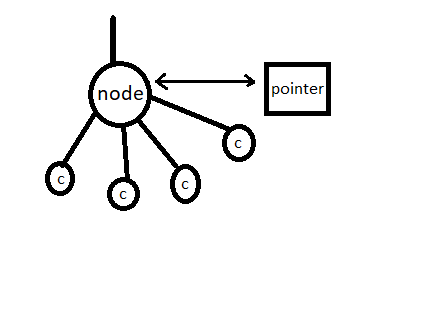
\includegraphics[width = 5cm]{images/29_1}

Если мы хотим перейти по указателю на какой-то узел, то мы ищем нужный pointer, в котором есть указатель на нужную нам вершину. И во время операции decreaseKey уменьшается ключ в нужной вершинке.
Для того чтобы поддерживать корректность ссылок между pointer и вершинами во время операций над кучей, будем действовать следующим образом: ( рассмотрим на примере siftUp)
\begin{figure}[h]
\center{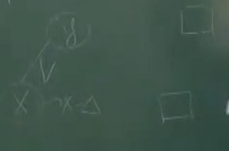
\includegraphics[width = 5cm]{images/29_2}}
\caption {У каждой вершины свой указатель, и надо сделать swap вершин}
\label{ris:image}
\end{figure}

\begin{figure}[h]
\center{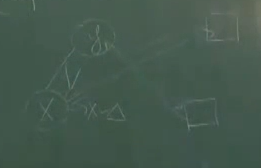
\includegraphics[width = 5cm]{images/29_3}}
\caption {Вторым шагом просто меняем указатели. И все становится вновь корректно}
\label{ris:image}
\end{figure}

Таким образом, для того, чтобы найти и изменить i-й добавленный элемент кучи, необходимо найти i-ую "коробочку" и перейти по указателю туда, куда она ссылается.

\section{Удаление из кучи по значению.}

Предположим, у нас есть некоторая куча H. И нам говорят: "Удалите элемент со значением 5". Чтобы выполнить этот запрос, мы заведем еще одну кучу deletedH, содержащую удаленные элементы H. Т.е. те, которые нам нужно удалить, но которые находятся где-то в куче на неизвестном месте. 
Заметим, что в куче есть только 2 операций, которые зависят от того, есть в куче "удаленные"  элементы или нет. Это getMin и extractMin. 
Модифицируем эти операции так, чтобы они работали корректно.

\textbf{1. ExtractMin }

Сначала необходимо проверить, не был ли минимальный элемент удален из кучи. Минимальный элемент в куче - это и минимальный элемент в куче удаленнных элементов. Если элемент уже удален, то просто удаляем минимальный элемент из обеих куч и пытаемся найти тот минимальный элемент, который еще не удален. Иначе удаляем только из текущей.

\textbf{2. GetMin }

Действуем аналогично. Если элемент уже удален, тогда мы удаляем его и пытаемся снова найти минимальный элемент в куче. Если элемент не удален, все хорошо, возвращаем минимальное значение

\section{Удаление из кучи по указателю}
Для того, чтобы удалить элемент из кучи по указателю, достаточно сделать decreaseKey( ptr, $\infty$). $\infty$ зависит от технической стороны вопроса. Если есть какое-то ограничение на числа в куче, то можно подобрать такое число, что после уменьшения на него элемент, на который ссылаются, станет минимальным в куче. Тогда достаточно сделать extractMin().

\begin{lstlisting}

void Heap::deletePtr(Node* ptr) {
	decreaseKey(ptr,  $\infty$);
	extractMin();
}
\end{lstlisting}

\textbf{Замечание:} Эта идея работает для любой кучи.